\section{Overview}

This thesis is concerned with solving one of the principal problems in the field of planet formation, how can we detect newly-formed planets, and measure their properties?
Answering these question is a vital step in constraining the various theoretical models of the planet formation process.

Stars and planets are born inside vast, interstellar clouds of gas and dust.
Sometimes called ``stellar nurseries'', these regions make up less than one percent of the interstellar volume of the Milky Way galaxy \citep{ferriere2001}.
Unlike the majority of the interstellar medium, which is ionised, the \textit{molecular clouds} of star-forming regions are composed primarily of gaseous H$_2$.
The typical size and mass range of these clouds are $2$ -- $15$ $\rm{pc}$ and $10^3$ -- $10^5$ $\rm{M_\odot}$ respectively \citep{cambresy1999}, where $\rm{M_\odot}$ is a solar mass.
Stars form as a result of the collapse of the cloud, either through gravitational instabilities \citep{jeans1902} or turbulent flows \citep{larson1981}.

The Solar System contains clues for how planets are subsequently formed around newborn stars.
The mass and angular momentum of the Sun and planets are segregated, with the Sun containing $99.86 \%$ of the total mass, and the orbits of the planets accounting for $98.5 \%$ of the total angular momentum \citep[e.g.][]{woolfson2000}.
Accounting for this proved to be a significant challenge for early models of the Solar System's formation, eventually culminating in the idea that the planets must have formed from a disk of gas and dust surrounding the Sun \citep[see review by][]{edgeworth1949}.
Such disks are known as \textit{circumstellar disks}, and they are a natural consequence of the star formation process; conservation of angular momentum prevents complete collapse, and instead a disk is formed \citep{terebey1984,shu1987}.
The outward transport of angular momentum and inward transport of mass is then facilitated by stresses and instabilities that operate within the disk \citep{lynden-bell1974,pringle1981}.
The disks found around young stars are thought to be the sites of planet formation, and are therefore known as \textit{protoplanetary disks}.

Protoplanetary disks have lifetimes on the order of a few Myr before they eventually disperse \citep[see review by][]{ercolano2017}.
Planets are formed some time during this period, although the efficiency of planet formation is not well known \citep[see review by][]{helled2014}.
\textit{Planetesimals} are formed in the disk through the repeated collision of dust and ice particles, resulting in the eventual formation of larger bodies.
Terrestrial planets, and possibly the cores of gas and ice giants, are then thought to form through the subsequent accretion of planetesimals and the surrounding gas and dust \citep[e.g.][]{johansen2014}.
Two competing models hope to explain giant planet formation, \textit{core accretion} \citep[CA;][]{lissauer1993,pollack1996,safronov1972} and \textit{gravitational instability} \citep[GI;][]{kuiper1951,cameron1978}.
CA provides a good explanation for the observed composition of the planets in the Solar System, as well as the known correlation between stellar metallicity and giant planet occurrence.
Notably, the formation timescale in this scenario is comparable to the lifetime of the disk.
On the other hand, GI allows planets to form essentially immediately, while the star is still embedded in its envelope.
However, it also faces challenges explaining the observed composition and correlations previously mentioned \citep[see review by][]{helled2014}.
Therefore, detecting and measuring the properties of newly formed planets while they are still in their natal disks will provide key constraints on these models, and provide insights into the physics driving planet formation.

\subsection{Protoplanet Detection}

\begin{figure}
    \centering
    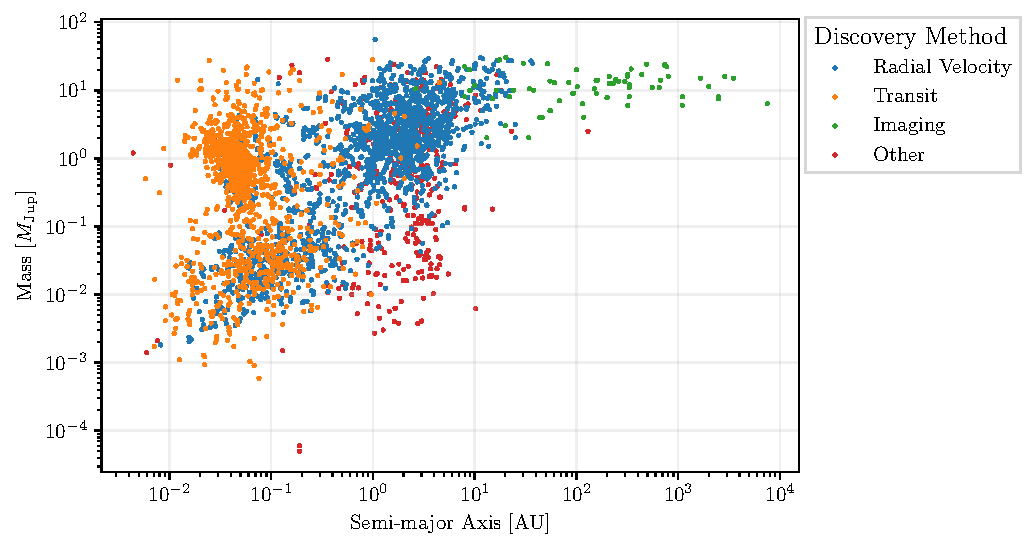
\includegraphics[width = 0.98\textwidth]{figures/exoplanet.pdf}
    \caption{Distribution of known exoplanet mass and orbital radii, coloured by detection method. Data taken from \textit{The Nasa Exoplanet Archive} \citep{nasa2022}.}
    \label{fig:exoplanets}
\end{figure}

The first planet outside our own Solar System, called an \textit{exoplanet}, was discovered in 1995 by Michael Mayor and graduate student Didier Queloz.
51 Pegasi b is a ``hot Jupiter'', with a mass of $\sim 0.5 \, \mathrm{M_J}$ and orbital period of $\sim 4$ days (where $\mathrm{M_J}$ is a Jupiter mass).
This places it nearly 20 times closer to its star, than the Earth is to the Sun \citep{mayor1995}.
In the nearly 30 years since that landmark discovery the number of confirmed exoplanets has skyrocketed to 5197 as of the time of writing \citep{nasa2022}.
The mass and orbital radius distribution of these planets is shown in Figure \ref{fig:exoplanets}.
Primarily, these detections have come from the transit and radial velocity methods.
The transit method relies on measuring the period dimming of star light as the planet passes between the star and observer, while the radial velocity method measures the doppler-shift of emission lines due to the motion of the star around the system barycentre.
Here, we are interested in the subset of exoplanets that have been detected while still embedded in their protoplanetary disks, so-called protoplanets.
Unfortunately, despite the other successes of exoplanet surveys, the number of uncontroversially confirmed protoplanets sits at an unimpressive total of two.
These are PDS~70 b and c, observed through direct imaging in the near-infrared \citep{keppler2018,haffert2019}.

Detecting protoplanets is a formidable task, owing to their environment.
The transit method is essentially unviable due to the presence of optically thick disk material in the system.
On the other hand, radial velocity searches are hampered by the high starspot and accretion activity of young stars, which complicates disentangling planet signals present in spectra \citep{desort2007}.
Furthermore, protoplanetary disks can have radii of hundreds of au \citep[e.g.][]{tripathi2017}, and so many protoplanets may sit outside the region of parameter space detectable by this methods anyway (see Figure~\ref{fig:exoplanets}).
Another popular technique, direct imaging (DI), is able to detect planets at these separations, but is not sensitive to planet masses under a few $\mathrm{M_J}$ \citep{jorquera2021}.
However DI has still seen some successes, the two aforementioned confirmed planets in the disk of PDS~70, as well as a host of further claimed detections in the disks of HD 100546 \citep{quanz2013}, HD 169242 \citep{biller2014}, LkCa15 \citep{sallum2015}, MWC 758 \citep{reggiani2018} and AB Aurigae \citep{currie2022}. Each of these are disputed in the literature \citep{rameau2017,ligi2018,currie2019} with the exception of PDS~70 b and c\footnote{AB Aurigae b is also currently not disputed in the literature but as of this writing the claimed detection is only 8 months old.}.
The main difficulty with DI the possible confusion of disk material with a planet, since processing techniques can create spurious point sources from filamentary substructures like arcs and spirals \citep[eg.][]{rameau2017}.

\begin{figure}
    \centering
    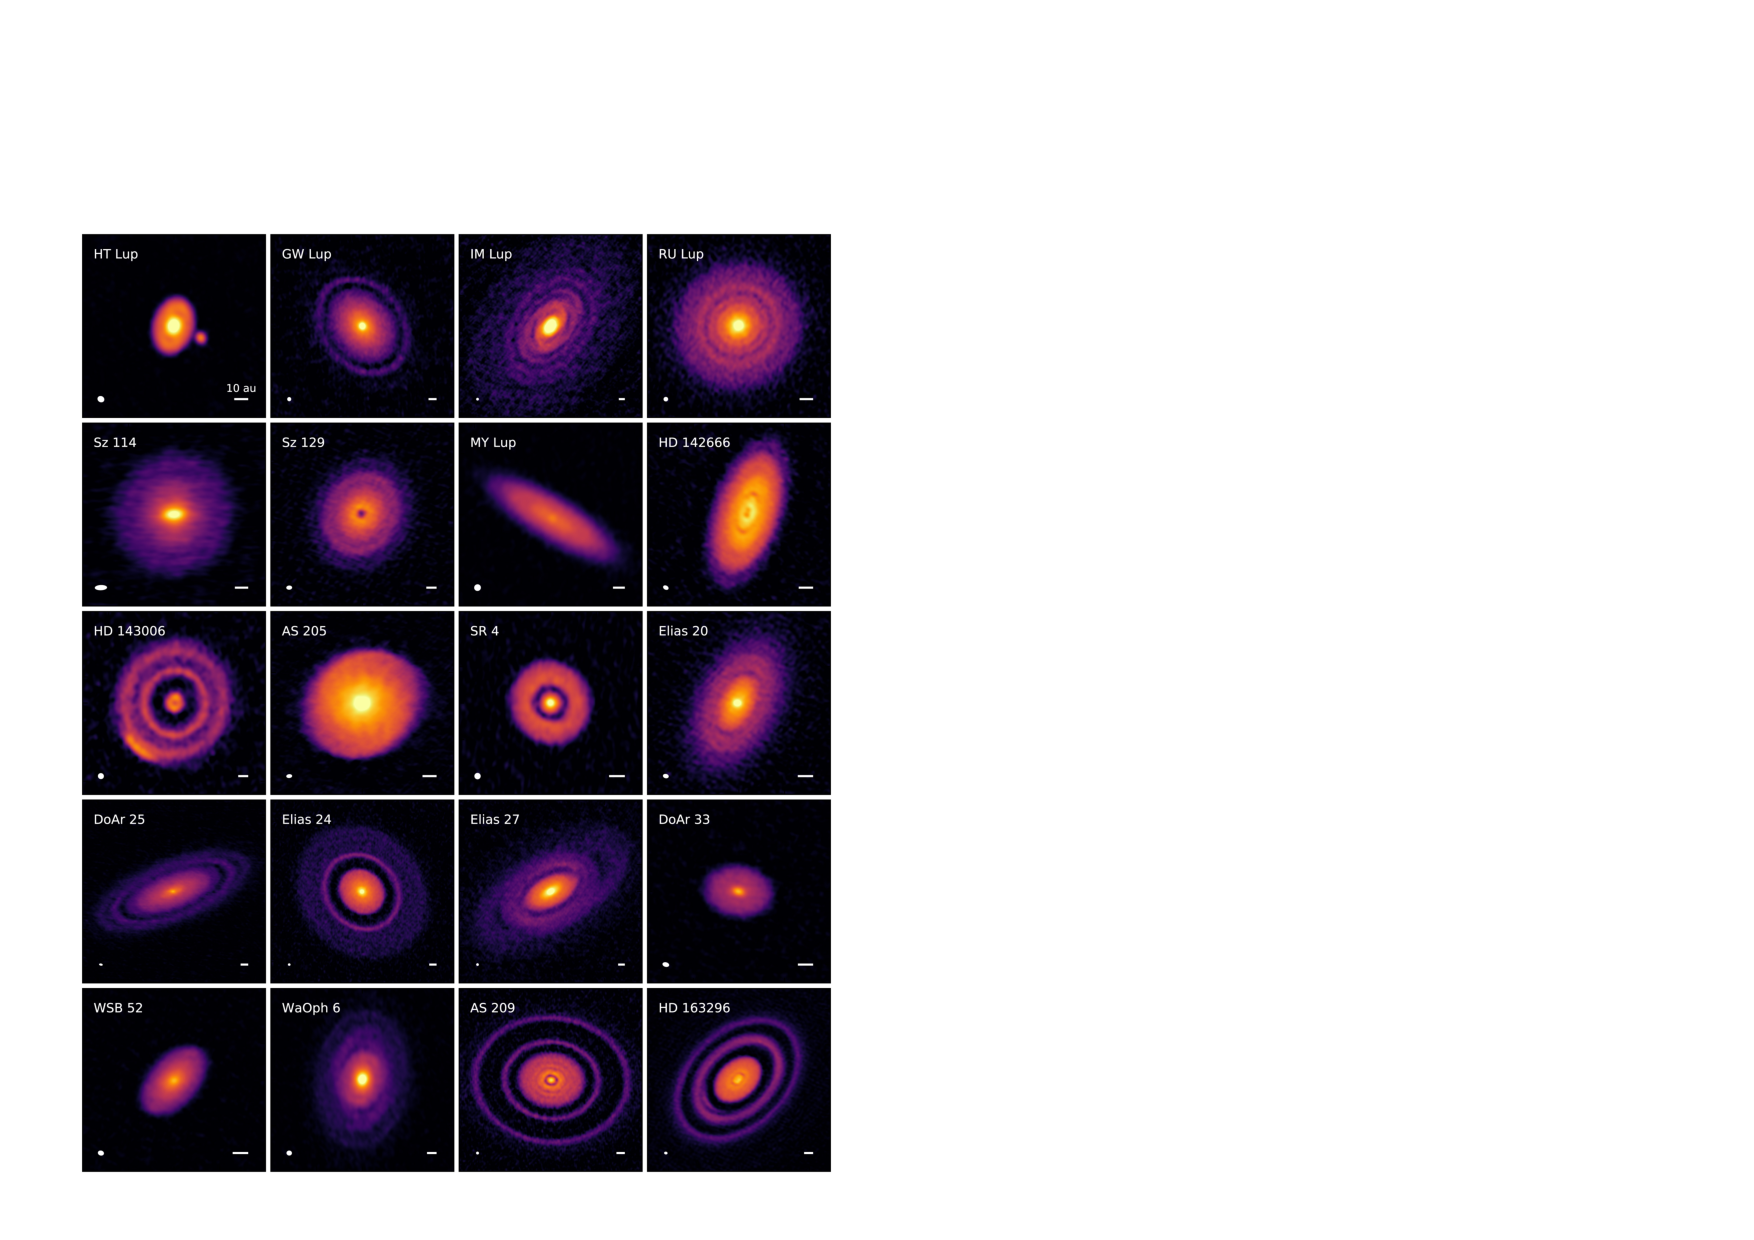
\includegraphics[width = 0.7\textwidth]{figures/DSHARP.pdf}
    \caption{Continuum images taken at 1.5 mm of the 20 protoplanetary disks in the DSHARP program. The colour scale has been stretched to increase the contrast. \citep{andrews2018}. Substructures are evident in each disk. Notable examples include: the thin and wide rings in AS 209 and HD 163296, spiral arms in IM Lup and Elias 2-27, and a bright arc in HD 143006.}
    \label{fig:DSHARP}
\end{figure}

\subsection{Disk Substructures}

The difficulty in looking for embedded planets directly motivates studying the interactions between embedded planets and their host disk, in hopes of observationally identifying signatures induced by the planet.
The foundations of our theoretical models for the interaction between a disk and an embedded gravitating body were developed in the late 70s by Peter Goldreich and Scott Tremaine, who were hoping to understand how Saturn's moons induce the spiral and concentric ring substructures within its rings \citep{goldreich1980}.
With the advent of the Atacama Large Millimetre Array (ALMA), we have begun to resolve the surfaces of protoplanetary disks at high resolution, and there we find evidence of the same kinds of interactions as those between Saturn's rings and moons.
Figure \ref{fig:DSHARP} shows continuum observations of 20 disks taken as part of the Disk Substructures at High Angular Resolution Project (DSHARP) \citep{andrews2018}.
All of the disks imaged show some sort of substructure, including bright and dark rings, spiral arms and bright arcs.
While alternative mechanisms have been suggested to drive such structures \citep[e.g.][]{kretke2007,simon2014,gonzalez2017}, the most popular explanation is that they are driven by embedded planets \citep{dipierro2015,dong2015b,bae2017,fedele2017,fedele2018,zhang2018}.
The observations provide evidence for early planet formation \citep{dipierro2015}, but they are far from a smoking gun due to the numerous proposed mechanisms that may create substructures in the absence of planets.
This thesis is concerned with disentangling these explanations, and confirming the presence of planets by instead looking for the characteristic way in which they perturb the velocity field of the disk.
That is, through observations of the disk \textit{kinematics}.

\section{Kinematic Observations}

\begin{figure}
    \centering
    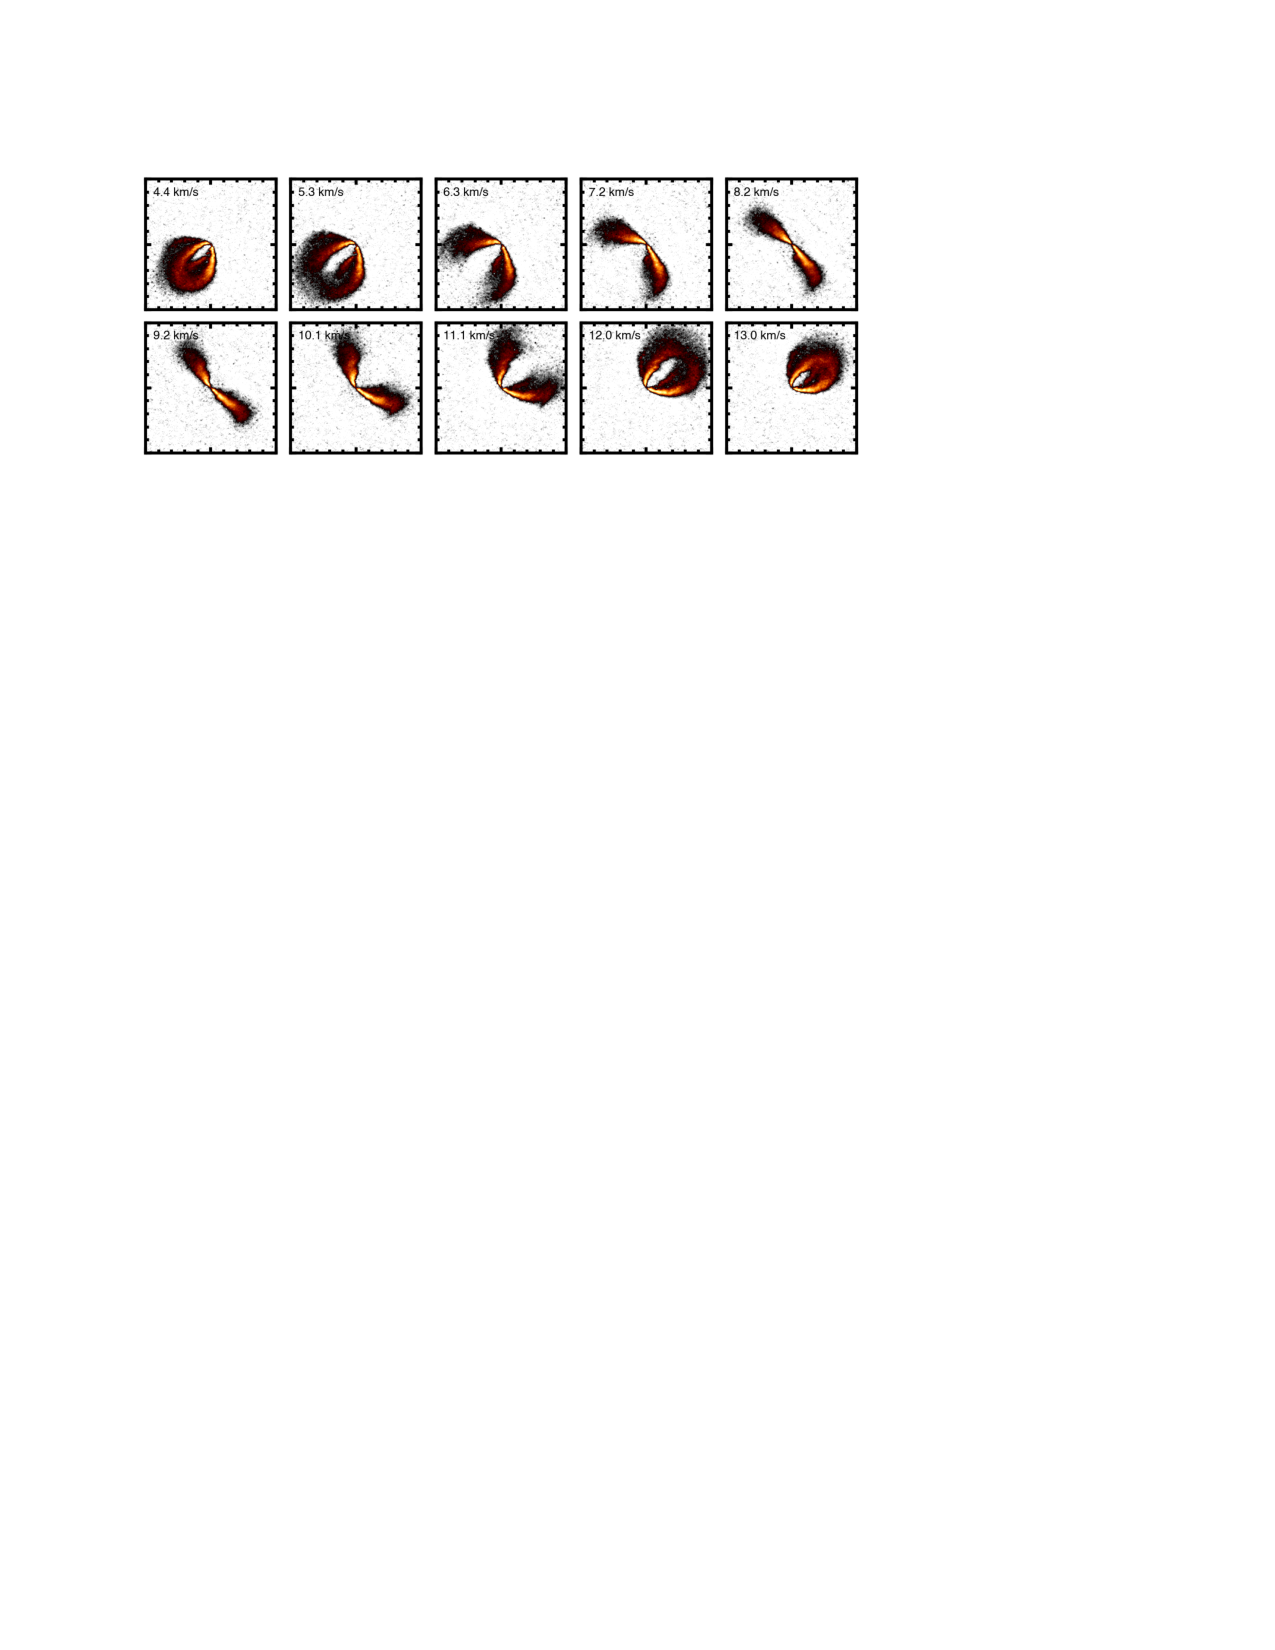
\includegraphics[width = 0.95\textwidth]{figures/channels.pdf}
    \caption{Velocity channels of $^{12}$CO emission from the disk around HD 163296 \citep{andrews2018}. The colour corresponds to brightness temperature, ie. brighter means more emission \citep{diskdynamicscollaboration2020}. Each channel probes the material in the disk moving at a certain velocity, resulting in the butterfly patterns seen across the channels. Note also that the CO emitting layer sits above the disk mid-plane, and so there is both a top and bottom surface in each image, with one surface mostly obscured by the other.}
    \label{fig:channels}
\end{figure}

The we may probe the kinematics of a disk by measuring the Doppler shift of spectral line emission from different molecules and their isotopologues\footnote{Isotopologues are molecules that are different only by the isotopes of their atomic components.}.
Such data come in the form of channel maps, which make up a data cube that has two spatial dimensions and one frequency dimension.
As it is the Doppler-shift of the line that is measured, the frequency dimension is equivalent to a velocity dimension.
Thus, taking a velocity slice of the cube yields an image of all the material in the disk moving with the same line-of-sight velocity relative to the observer.
The frequency dimension is equivalent to velocity, and so in each frequency slice we find an image of all the material with the same line-of-sight velocity.
Figure \ref{fig:channels} shows velocity channels of $^{12}$CO $J=2-1$ rotational line emission from HD 163296, imaged with ALMA \citep{andrews2018}.
The observations show the expected butterfly shape that is characteristic of Keplerian rotation \citep{degregorio-monsalvo2013}.
Note also that since $^{12}$CO line emission occurs at multiple scale heights, there is a top and bottom surface in each image.
Since velocity channels probe the material moving at a certain line-of-sight velocity, the maximum emission in each channel should trace an iso-velocity contour.
These iso-velocity contours are the lines of constant line-of-sight velocity, and they should be continuous and smoothly varying for Keplerian rotation.

\begin{figure}
    \centering
    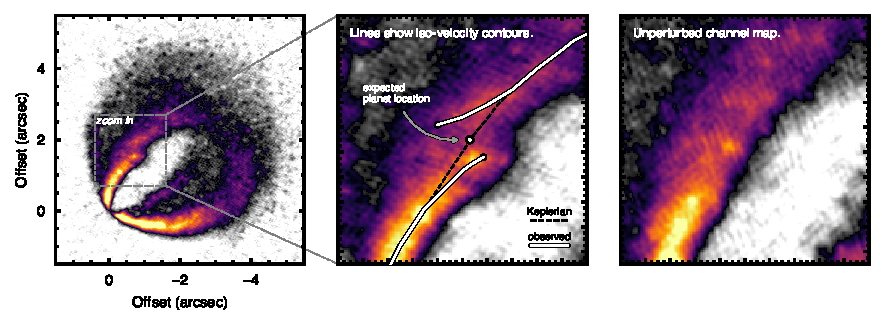
\includegraphics[width = 0.98\textwidth]{figures/HD163296_channels.pdf}
    \caption{A close view of the $12 \,\mathrm{km/s}$ velocity channel of HD 163296 \citep{andrews2018}, highlighting the velocity kink found by \citet{pinte2018a} Comparing the middle and right panels, we see how the line of maximum emission deviates from the iso-velocity contour expected from pure Keplerian rotation. \citep{diskdynamicscollaboration2020}.}
    \label{fig:velocity_kink}
\end{figure}

Figure~\ref{fig:velocity_kink} shows a zoomed in view of one of the channels in HD~163296, highlighting the localised deviation from Keplerian rotation first found by \citet{pinte2018a}.
Such deviations are called ``velocity kinks'', and \citet{pinte2018a} found that it matched the expected signature that should be produced by the gravitational disturbance of an embedded planet \citep{perez2015}.
Through hydrodynamical modelling and radiation transfer simulations, \citet{pinte2018a} showed that the density waves generated by such a planet can accurately recreate the observed kink.
A comparison of their simulations with the observations is shown in Figure~\ref{fig:pinte2018_hydro}.
A similar velocity kinks was also found in the disk of HD~97048, and again detailed simulations show that a planet of a few $\mathrm{M_J}$ is capable of recreating the observations \citep{pinte2019}.
A follow up survey of the disks in the DSHARP sample found kinks in 8 out of 18 disks \citep{pinte2020}.
Importantly, in the case of all the aforementioned disks, all of the candidate protoplanets lie within an observed dust gap or at the end of a spiral arm detected in continuum emission \citep{huang2018b,huang2018,pinte2020}.

\begin{figure}
    \centering
    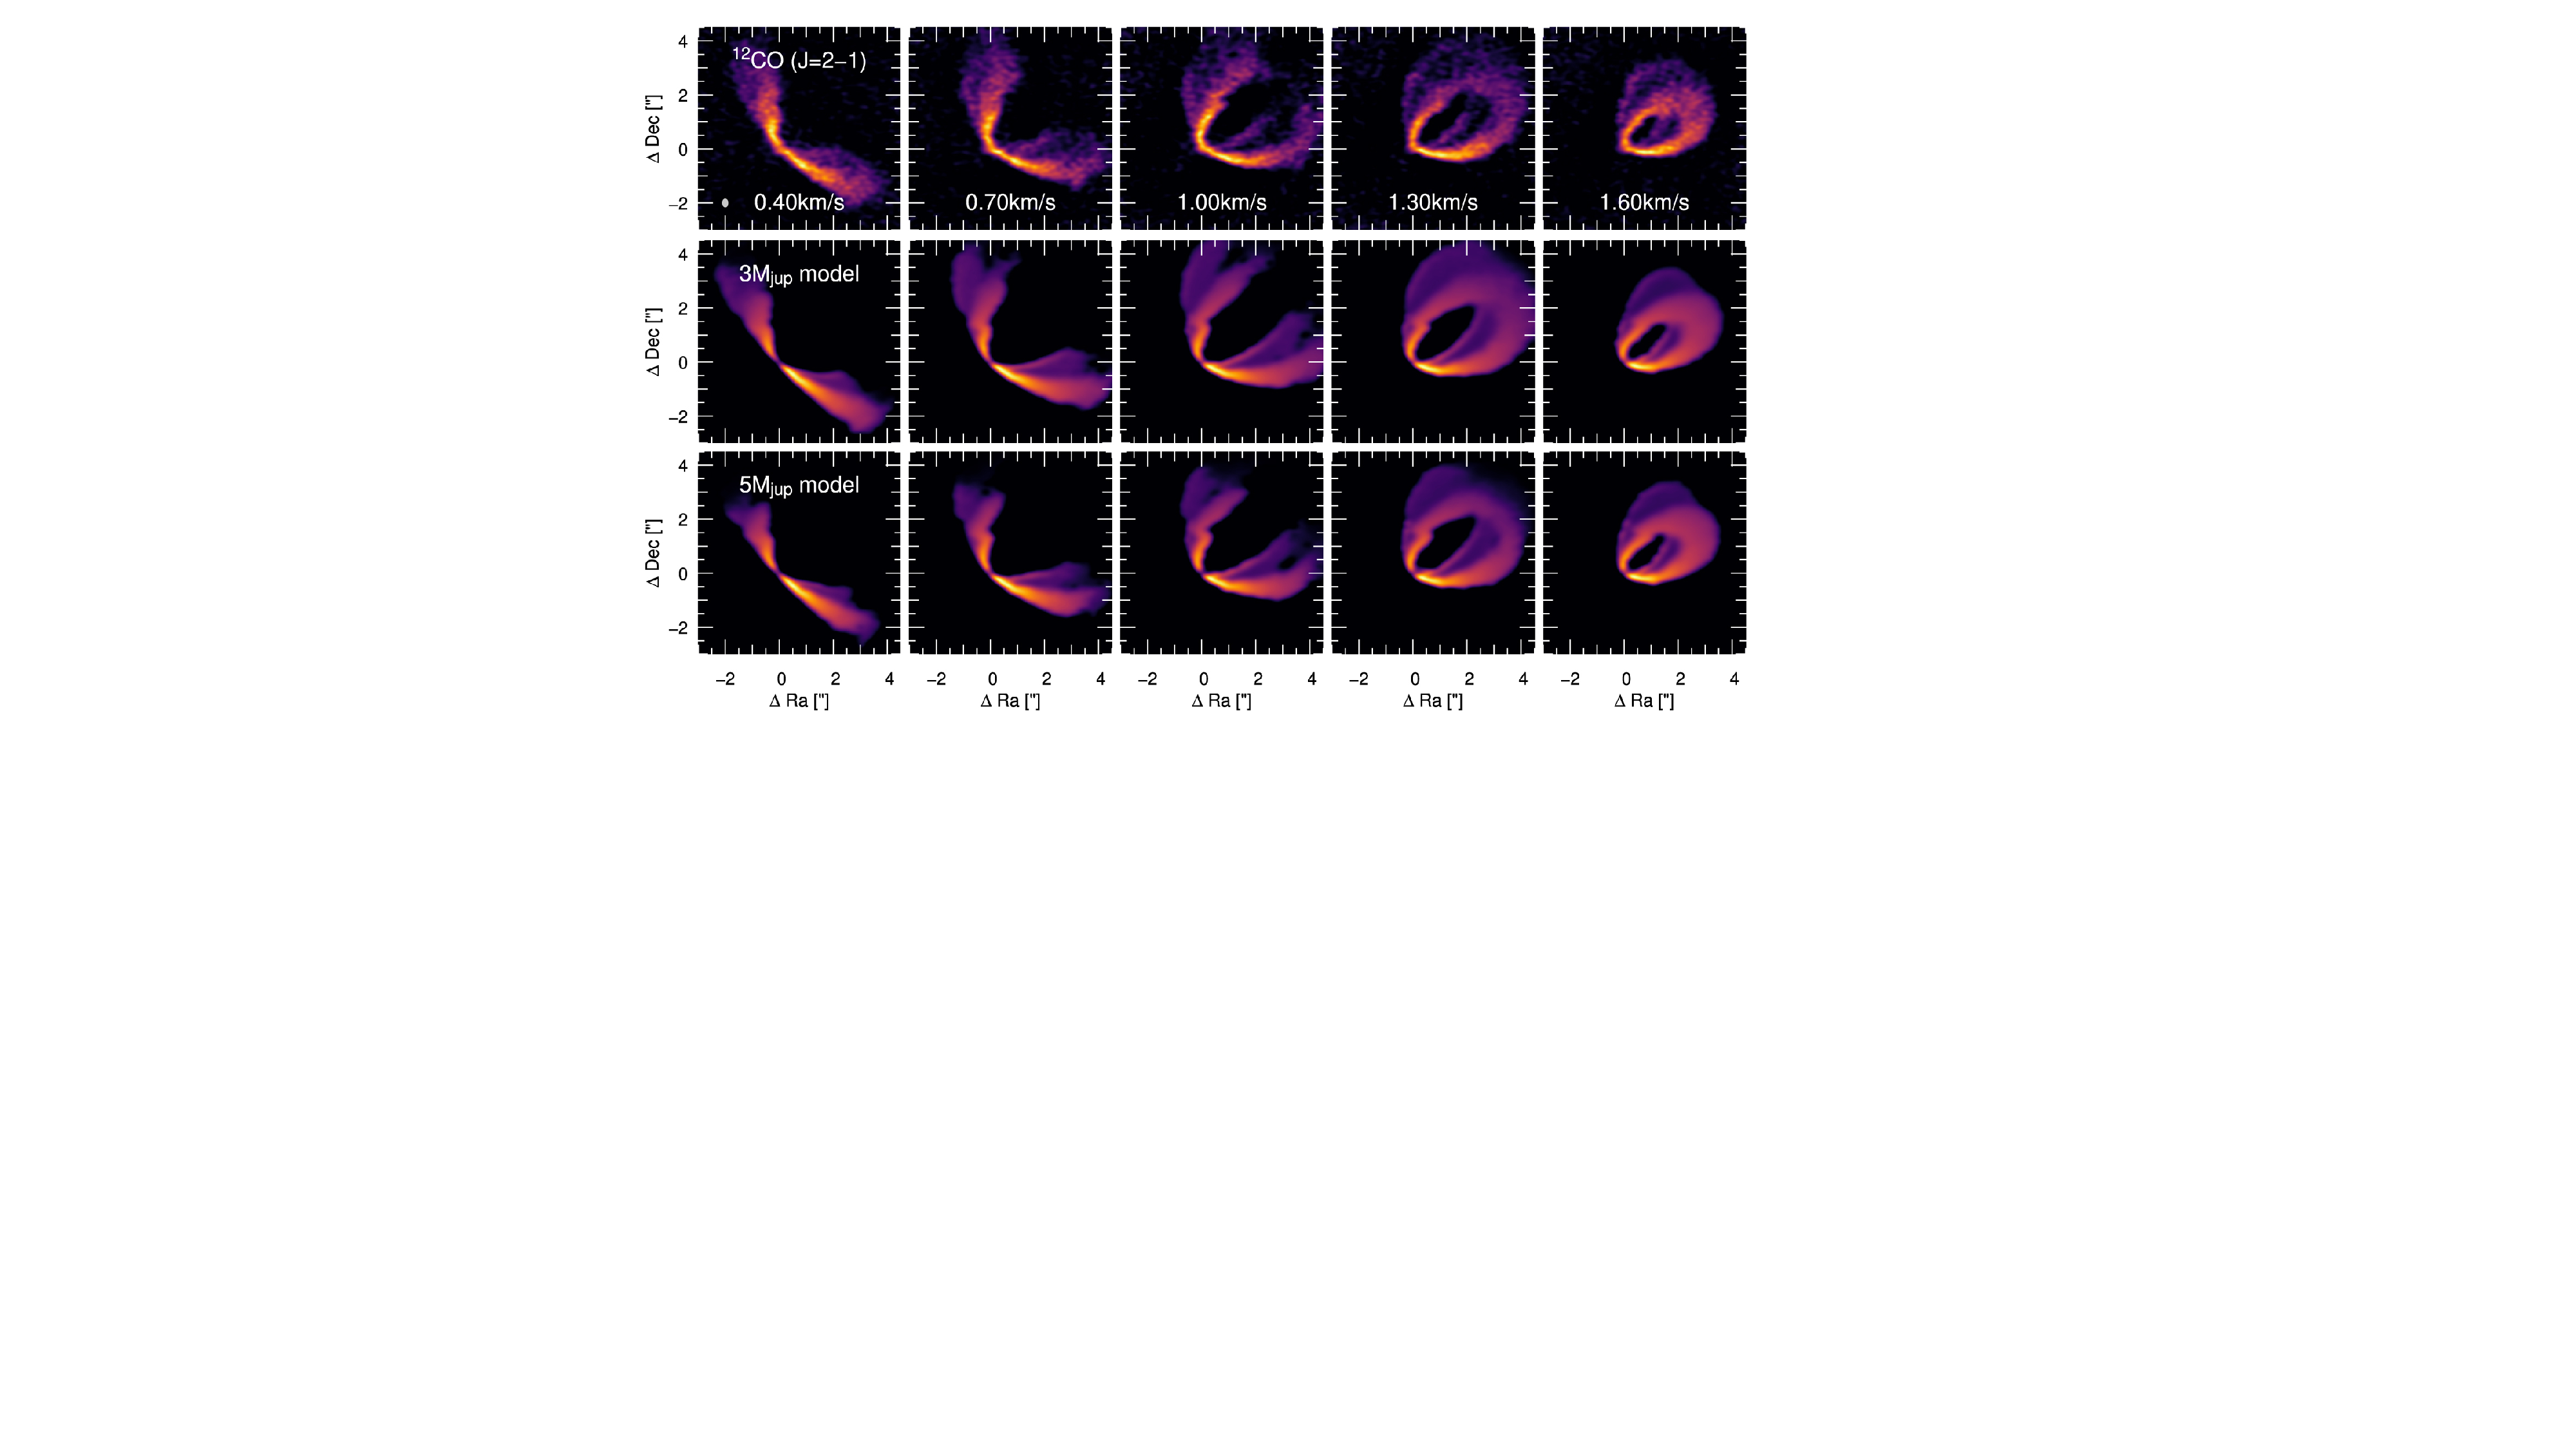
\includegraphics[width = 0.98\textwidth]{figures/pinte_2018_sims_channels.pdf}
    \caption{Comparison of $^{12}$CO ALMA observations (top row) with the synthetic channel maps created from 3D hydrodynamical simulations of planet-disk interactions by \citet{pinte2018a}. The synthetic images were convolved with a Gaussian to match the beam size of the observations.}
    \label{fig:pinte2018_hydro}
\end{figure}

Further kinematic evidence for planets has been found through using the channels maps to calculate the velocity field of the disk, and then subtracting the best-fitting background rotation to generate residuals.
\citet{casassus2019} and \citet{perez2020} used this technique to identify a ``Doppler flip'' in the disk of HD~100546, where the velocity abruptly changes sign over the planet location.
Furthermore, the high angular resolution gas observations taken as part of the Molecules with ALMA at Planet-forming Scales (MAPS) survey have allowed for detailed mapping of the kinematics disks around HD~163296 and MWC~480, with multiple spiral and arc structures detected \citep{teague2021}.
A similar analysis was performed with ALMA observations of TW~Hya, with the authors claiming the detection of one large, coherent spiral structure \citep{teague2022}.

Such kinematic observations provide support for the planet-disk interaction picture for disk substructures. Furthermore, they allow for the constraint of the planet mass through modelling of such interactions, as shown by \citet{pinte2018a,pinte2019}.
However, the computational cost of full 3D hydrodynamical simulations prohibits their use as part of a robust fitting procedure.
While statistical tools have recently shown promise in detecting and constraining planets through kinematics \citep{izquierdo2021,izquierdo2022}, it would be valuable to do this through the physics of the interaction.

\subsection{Semi-Analytic Models}

Recently, \citet{bollati2021a} developed a theoretical framework for understanding velocity kinks through the creation of semi-analytic models of the planet wake.
This work was based on the linear theory for the density waves excited in a disk by a gravitation body \citep{goldreich1980}, as well a weakly non-linear theory for subsequent steepening into shock waves \citep{goodman2001,rafikov2002a}.
In their view, velocity kinks are caused by these density waves perturbing the velocities of the disk, and they found that measuring the amplitude of the kinks should provide the necessary information needed to recover the planet mass.
However, the mass obtained is in units that are very sensitive to the temperature structure of the disk, and so a robust planet mass measurement requires a tight constrain of this structure.
They also found that velocity kinks arise due to the intersection of the planet wake and the velocity channels, and that these kinks are spread throughout the disk.
Since at the time kinks were thought to be localised nearby the planet \citep{pinte2018a,pinte2019,pinte2020}, Bollati suggested that viscous damping may suppress the amplitude of the wave as it travels through the disk.

In \citet{calcino2022}, we found that the HD~163296 is indeed host to many velocity kinks far from the proposed planet location by using high resolution data from the Molecules with ALMA at Planet-Forming Scales program \citep[MAPS;][]{oberg2021}.
Using this, we traced the outer planet wake through the disk, directly confirming the presence of a Lindblad planet wake for the first time.
Figure \ref{fig:wake_channel} shows how this wake gives rise to the observed velocity kinks as it passes through the velocity channel.
This work thus showed that the wake-crossing interpretation of velocity kinks of \citet{bollati2021a} is indeed correct, and that there is no need for any damping.
Importantly, the shape of the wake depends on the disk temperature, and so mapping the wake constrains the temperature structure of the disk, and so determines the unit for the planet mass.

Taken together the work presented in \citet{bollati2021a} and \citet{calcino2022} provide the necessary ideas needed to recover a planet mass from observations of disk kinematics, by measuring both the amplitudes of velocity kinks, and the shape of the planet wake.
This thesis builds on their work, by taking further steps towards the creation of a fitting procedure to do just this.

The structure of the thesis is as follows:
\begin{itemize}
    \item Chapter 2 discusses the properties and structure of protoplanetary disks, from both a theoretical and observational point of view.
    \item Chapter 3 provides a theoretical overview of the planet-disk interaction, as well as the particular ideas behind the semi-analytic models.
    \item Chapter 4 presents our Python package for generating models of the planet wake excited by a planet embedded in a disk, and discusses our numerous improvements over the methods of \citet{bollati2021a}.
    \item Chapter 5 presents an application of the semi-analytic models in conjunction with hydrodynamical models, to map the planet wake in kinematic observations of HD~163296.
    \item Chapter 6 presents two further applications of the models, for kinematic planet detection in the disks of HD~169142 and IM~Lupi.
    \item Chapter 7 presents our preliminary work on developing a fitting procedure to recover planet masses from kinematic observations using the semi-analytic models.
\end{itemize}

\begin{figure}
    \centering
    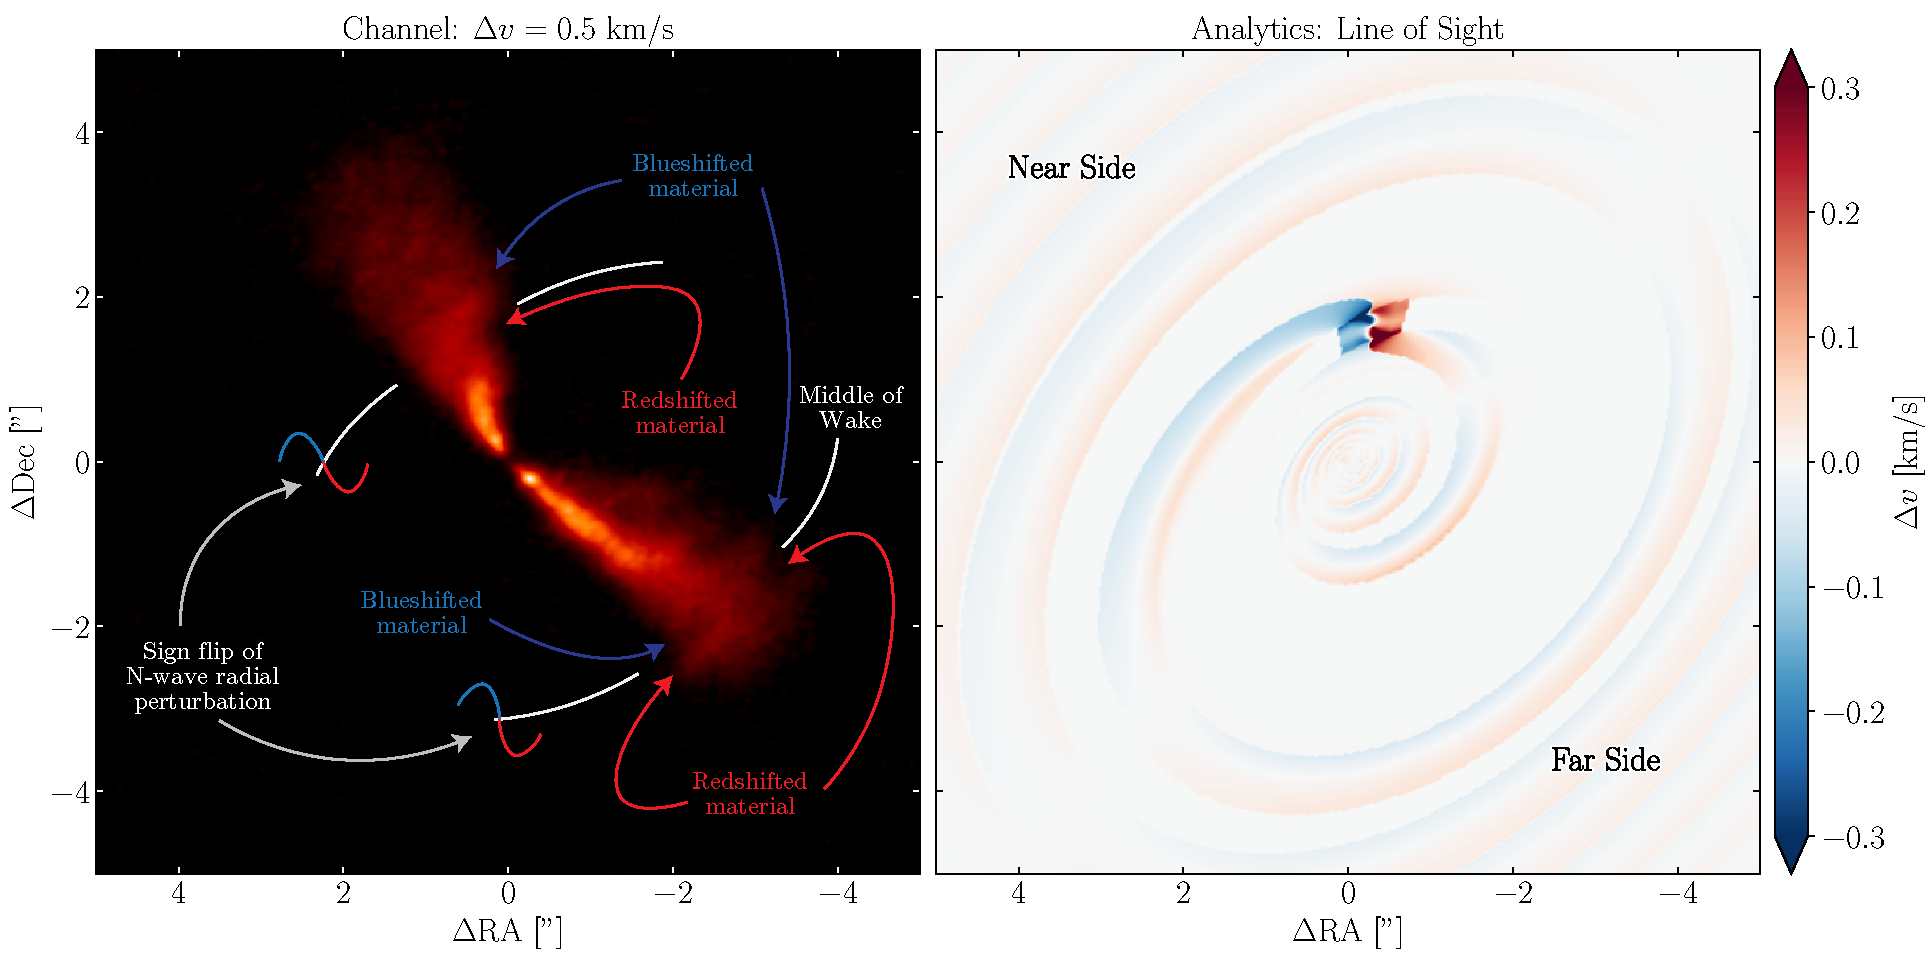
\includegraphics[width = 0.95\textwidth]{figures/labeled_channel.pdf}
    \caption{Comparison of one of the velocity channels of HD 163296 observed as part of the MAPS program \citep{oberg2021}, with the analytic model \citep{bollati2021} of the proposed planet wake created by \citet{calcino2022}. The observed kinks on each side of the disk are well explained by the crossing of the planet wake with the channel, as in \citet{bollati2021}.}
    \label{fig:wake_channel}
\end{figure}